\chapter{Generative Adversarial Networks (GAN)}

\section{Introduction}
Till now we have focused our attention on \textit{discriminative models} that roughly speaking, given some data in a given space $x$, gives by a certain \textit{probability distribution} the information on which class $y$ they are part. There are plenty of machine learning techniques that solve effectively this type of task. These models are seeking in \underline{existing data} some interesting patterns and use them in order to predict a class (classification) or a continuous number (regression).\\
At the opposite \textbf{generative models} given a noise input $z$ and a certain class $y$, generate a new, never seen sample $x$ for that class. In this chapter, in particular we are going to talk about \textit{GANs (Generative Adversarial Networks)} which were invented by a PhD student (Ian Goodfellow), this enabled computers in the generation of new data using not one, but \textbf{two different neural networks}. 

\begin{figure}[h]
    \centering
    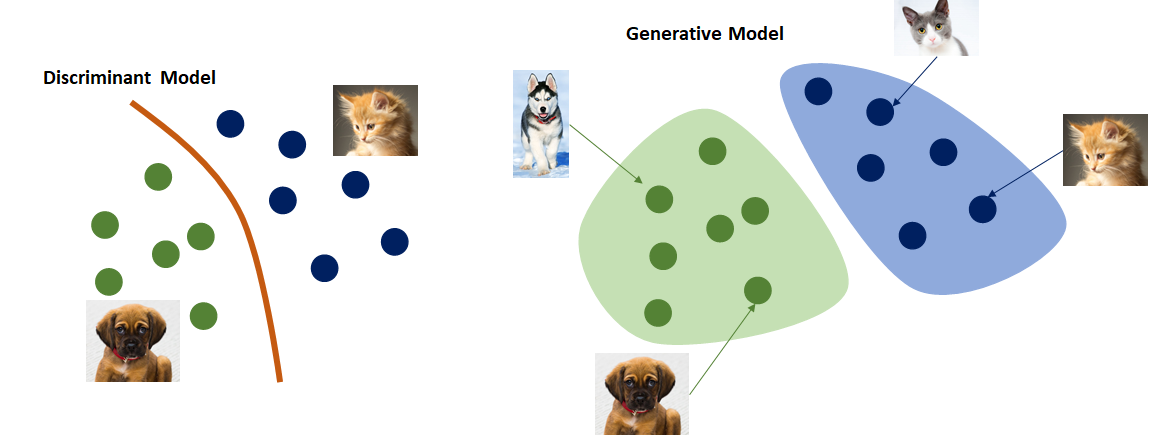
\includegraphics[scale=0.3]{img/generative_1.png}
    \caption{Discriminative vs Generative Models}
\end{figure}

\section{Variational Auto-Encoders (VAE)}
We consider here as a first approach to generative models the \textbf{autoencoders} and \textbf{variational autoencoders}, for several reasons: (i) it is an easier setting for generative AI; (ii) since generative models are challenging to be understood, autoencoders are closer to the models we have already seen, (iii) the autoencoders are directly or implicitly used in some variants of GAN architectures.

\subsection{Autoencoders}
The structure of an autoencoder is quite intuitive and follows these few steps: 
\begin{enumerate}
    \itemsep-0.3em
    \item \textsc{Encoder Network} this is the stage where we take a (full) representation $x$ (of an image for example) and reduce its dimension into a space $z$ by using a \underline{learned} encoder (a  classical ConvNet for example); 
    \item \textsc{Latent space} this is an intermediate stage in which the autoencoder architecture tidies its \textit{thoughts}; 
    \item \textsc{Decoder Network} we reconstruct the original dimension of the input $x$, starting from the latent space into a new generated image we call $x^*$.
\end{enumerate}

\begin{figure}
    \centering
    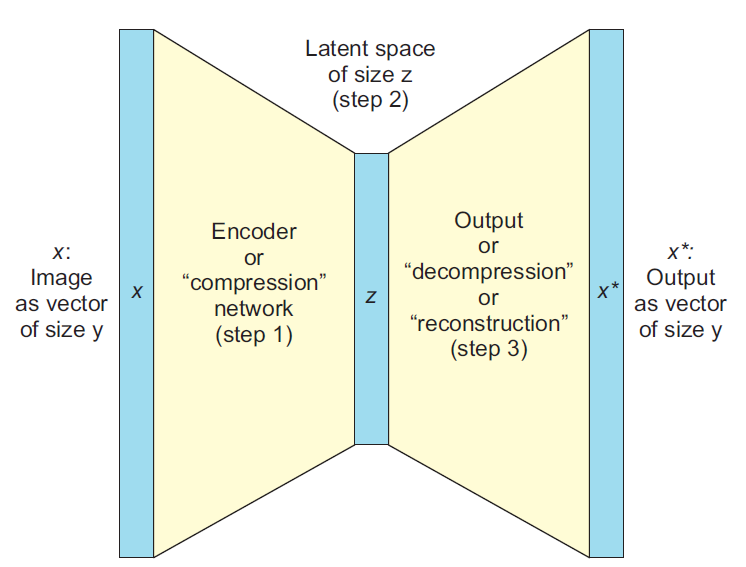
\includegraphics[scale=0.5]{img/autoencoder.png}
    \caption{Autoencoder architecture}
\end{figure}

\noindent
The \textit{training of an autoencoder} occurs as follows: 
\begin{enumerate}
    \itemsep-0.3em 
    \item We take the images $x$ through the autoencoder; 
    \item We collect the generated images $x^*$ as reconstruction of the given images;
    \item We measure a form of \textit{reconstruction loss} by mean (for example) of a mean squate error between the pixels of $x$ and $x^*$
    \item We obtain an explicit objective function to be minimized by mean of a gradient descent approach:
    \begin{equation}
        \mathcal{L}=\Vert x-x^* \Vert_2^2 
    \end{equation}
\end{enumerate}
The autoencoders can work by mean of an unsupervised machine learning model where we learn only from the training data without the labels. Note that we have a single loss function to be optimized with the common goal of \textit{minimizing the differences between the input and output images}.
We can use an autoencoder for different purposes, for example: image denoising, image colorization... 

\subsection{Variational autoencoders}
The traditional autoencoder maps the features of the input space into a latent space where the representation $z$ is nothing but a set of numbers. The main difference between autoencoders and Variational autoencoders (VAE) is just on the "magic" latent space. In fact here the choice is to represent the latent space as a \textit{probability distribution} with a certain mean ($\mu$) and a standard deviation $(\sigma)$. Note that you have to learn such a distribution! Once you have the distribution, you sample some numbers from it, add some noise and feed them to the decoder that will generate something that looks like the images of the training set, with the only difference they are \textbf{newly generated}. 

\begin{figure}[h]
    \centering
    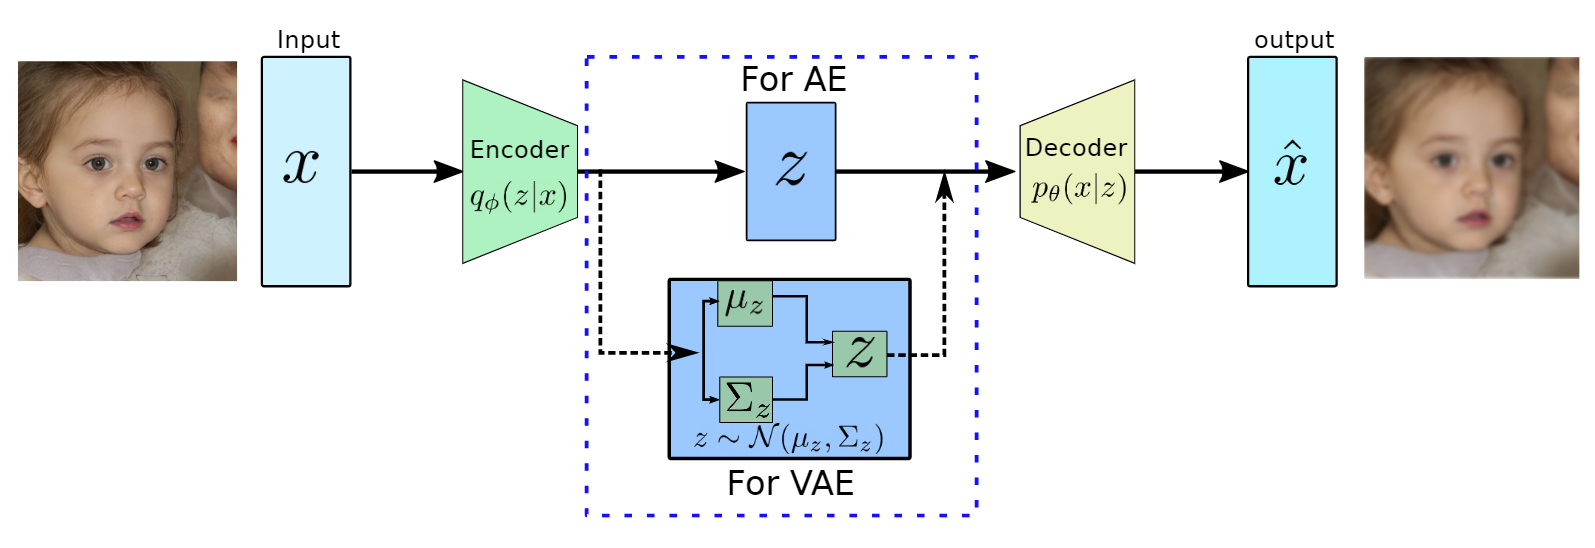
\includegraphics[scale=0.7]{img/VAE.png}
    \caption{(Variational) Auto-Encoder}
\end{figure}

\section{Generative Adversarial Networks}
\textbf{\textit{Generative Adversarial Networks} (GANs)} constitute a class of machine learning techniques which consist of two jointly trained models: the first (the \textit{Generator}) trained to create (generate) fake data, and the other (the \textit{Discriminator}) trained to binary distinguish fake data from real data. Let us go more deeply in the description of the GAN term:
\begin{description}
    \item[GENERATIVE] is the overall purpose of the machine learning model: generate new data. Clearly the generated data (images for example) depends on the features of the training set. If we want to generated new pictures of Leonardo Da Vinci, we must have a training set with Leonardo Da Vinci's portrait.
    \item[ADVERSARIAL] term refers to the game-like, competitive dynamic between the two models that constitute such a framework: the Generator and the Discriminator. The form is like an \textit{art forgery} while the discriminator is like an \textit{art expert} whose role is to say wheter a painting is fake or real; 
    \item[NETWORK] the models used for representing the two counterpart of the architecturesare neural networks. According to the complexity of the model, these can be simply Fully Connected Network, or ConvNet or in even more complex cases architectures like U-Net.   
\end{description}

This vanilla architecture is not suitable when: 
\begin{enumerate}
    \item We have large variations and different classes, while it performs well with small variations and small datasets;
    \item In such a type of architecture there is no way to control what the network have to generate.
\end{enumerate}
Both these issues are addressed introducing some novel aspects in the basic architecture, how we will see in the next sections.\\
Nowadays, GANs are used in order to synthetize artificially some images of some class or for other purposes like text to image or image to image translation. It is remarkable that for GAN there is not a latent space that will be decoded into a generated sample, due to the presence of a discriminator that allows the generator to be improved.

\begin{figure} 
    \centering
    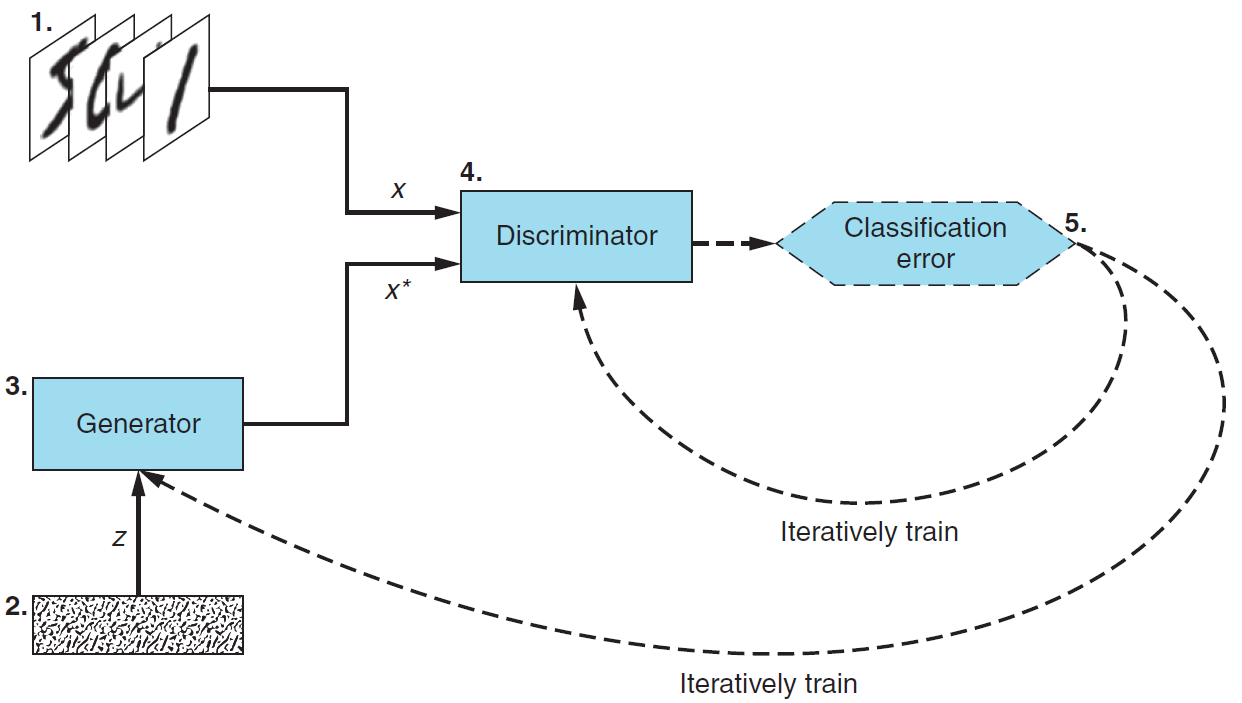
\includegraphics[scale=0.6]{img/GAN_1.png}
    \caption{GAN architecture}
    \label{fig:GAN_arch}
\end{figure}

\subsection{GAN anatomy}
The \Cref{fig:GAN_arch} shows the architecture of a GAN in its original form. Let us analyze the details of such diagram: 
\begin{enumerate}
    \itemsep-0.2em
    \item \textit{Training dataset} these are the real examples from which we want to learn the features, this is the input $x$ to the discriminator network
    \item \textit{Random noise vector} Is the input $z$ of the Generator network, is nothing but a vector of random number that the generating network uses as a starting point;
    \item \textit{Generator network} Takes as input the noise vector $z$ and outputs fake samples $x^*$, its goal is to produce samples that are as close as possible to the real data in order to fool  the Discriminator; 
    \item \textit{Discriminator network}  takes as input either a real example $x$ or a fake one $x^*$, for each generated example the Discriminator determines and outputs the probability of wheter an example is real/fake.
    \item \textit{Iterative training tuning} where the Discriminator's weights and biases are update in order to maximize the classification accuracy (maximizing the probability that $x \to${real} and $x^* \to$ fake), while the Generator's weights and biases are updated in order to maximize the probability that the discriminator classify $x^*$ is real. This is the reason why the two networks are as in a competition.
\end{enumerate}
Now we can say that: (i) at the end of the training the discriminator models $p(y|x)$ where $y$ can be real or fake; (ii) the generator learns a certain probability $p(x|y)$ that depends on the characteristics of the training set, that is the most common examples in the training set will be the most likely to be generated.\\

Note that the discriminator is used only in training phase: once you have obtained the learned generator, it is sufficient to provide it some noise vectors that will be mapped into generated images.

\subsection{Training GAN}
Till now we have done a snapshot of the engine analyzing the main features and the components it is made up of. An explanation of the training process is given here in order to better understand the mechanisms under the hood. The training of a GAN sees the alternate tuning of the Discriminator and Generator. In particular: 
\begin{enumerate}
    \itemsep-0.3em
    \item \textsf{Train the Discriminator}
    \begin{itemize}
        \itemsep-0.3em
        \item[a] Take a random real example $x$ from the training dataset; 
        \item[b] Get a random noise vector in order to generate a fake example $x^*$; 
        \item[c] Use the Discriminator to classify $x$ and $x^*$
        \item[d]  Compute the classification error (loss) and backpropagate the total error in order to update the Discriminator trainable parameters, seeking to minimize the classification errors;   
    \end{itemize}
    \item \textsf{Train the Generator}
    \begin{itemize}
        \itemsep-0.2em
        \item[a] Get a random vector $z$ and using the Generator Network we synthetize a new fake example $x^*$;
        \item[b] Use the discriminator to clasify $x^*$
        \item[c] After having computed the classification (loss function), backpropagate the error in order to update the Generator's learnable parameters in order to maximize the classification error.  
    \end{itemize}
\end{enumerate}
These two steps are repeated for each iteration. The alternate training of both models, these are supposed to improve together! Indeed, a perfect discriminator will not permit the generator to improve, a perfect generator model will always fool the discriminator without allowing it to improve. In the following we will indicate the elaboration of an image through the discriminator as $D(x)$ or $D(G(z))$ (in the first case it takes a real example in the second case a generated one), the elaboration carried out by the generator are indicated with $G(z)$ (where $z$ is a noise vector).
Next, we are going to enter moore deeply into the GAN formulation including the cost function and possible stopping criteria to learning.

\subsection{GAN Formulation}
A Generative Adversarial Networks model can be formulated as a \textbf{min-max game} where the discriminator is trying to maximize its reward, while the generator is trying to minimize such reward. That is
\begin{equation}
    \min_{G} \max_{D} V(D,G)
\end{equation}
where
\begin{equation}
    V(D,G)=\mathbb{E}_{x\sim{p_{data}(x)}}[\log(D(x))]+
    \mathbb{E}_{z\sim{p_{g}(z)}}[\log(1-D(G(z)))]
\end{equation}
we take the \textit{expected values} since both $x$ and $z$ are random vectors. From such a $V(D,G)$ we are able to extract the loss functions $J^D$ and $J^G$ for the discriminator and generator according to the objective we have stated about them.

\subsubsection{Discriminator loss function $J^D$ and gradient ascent}
It is required that the Discriminator predicts 1 for real image, 0 for fake ones, it is sufficient to impose
\begin{equation}
    J^D = V(G,D)
\end{equation}
since the first term is maximum when $D(x)=1$ ($D$ applied to the real example $x$ gives 1 (real)) and the second term is maximum when $D(G(z))=0$ (that is $D$ applied to the generated example $G(z)$ gives 0 $\to$ fake). The \textbf{gradient ascent} algorithm can be used so that the parameters $\theta_d$ are updated as:

\begin{equation}
    \theta_d \leftarrow \theta_d + \mu \nabla{J^D}(\theta_d)
\end{equation}
with $\mu$ being the learning rate.

\subsubsection{Generator loss function $J^G$  and gradient descent}
Since the generator needs to fool the discriminator it must update its own parameters so that the discriminator could predict 1 when $G(z)$ is provided. The second term of $V(G,D)$ is taken as $J^G$ since it is the one in which the $G(z)$ appears. Then: 
\begin{equation}
    \mathbb{E}_{z\sim{p_{g}(z)}}[\log(1-D(G(z)))]
\end{equation}
such a functional is minimum when $D(G(z))=1$. Since we want to minimize $J^G$, \textbf{gradient descent} must be applied: 
\begin{equation}
    \theta_g \gets \theta_g  - \mu \nabla{J^G}(\theta_g)
\end{equation}
with $\mu$ being the learning rate.\\

An alternative formulation, called the \underline{Non-Saturating GAN}, sees the generator to maximize the log-probability that the discriminator could fail. 

\subsection{When to stop training GAN?}
Those familiar with \textit{game theory} will recognize that the GANs can be seen as a \textit{zero-sum game}, where there is at a certain point a \textbf{Nash equilibrium point}. This can be reached either when the generator has the same distribution of data with respect to the discriminator, or when the discriminator always outputs a probability of 1/2 for each given sample. In this situation neither player can improve its own position.

\subsection{The challenges in Training GAN}
We have understood that training a GAN is not so simple, since the two networks are in competition the one with another. Moreover the training is even more \textbf{challenging} due to two main reasons: (i) Non convergence; (ii) Mode collapse.

\subsubsection{Non-convergence}
The deep-learning model we have seen before introducing GANs involved a single player that has been trying to maximize its reward, we used Stochastic Gradient Descent that guaranteed convergence under certain conditions. In the case of GANs there is a player which is trying to minimize the reward of the other. There is no collaboration, moreover the gradient based method are not converging to the Nash Equilibrium.

\subsubsection{Mode collapse}
We refer to \textbf{mode collapsing} to indicate a failure where the generator model in the GAN produces only a \textit{limited variety of output} neglecting the diversity which is present in the dataset with real samples, and then in the data distribution. This can lead the generator to produce  \textit{few modes} or a \textit{single one}. Why does this phenomenon occur? It is mainly related to the \textit{adversarial dynamics} underlying the GAN formulation and the minimax game: if the generator (G) finds that the discriminator (D) is fooled when producing examples of a certain mode, then the generation goes toward the direction of producing images of that modes which, anyway maximize the classification error of D. We show an example of this fact: 

\begin{figure}[h]
    \centering
    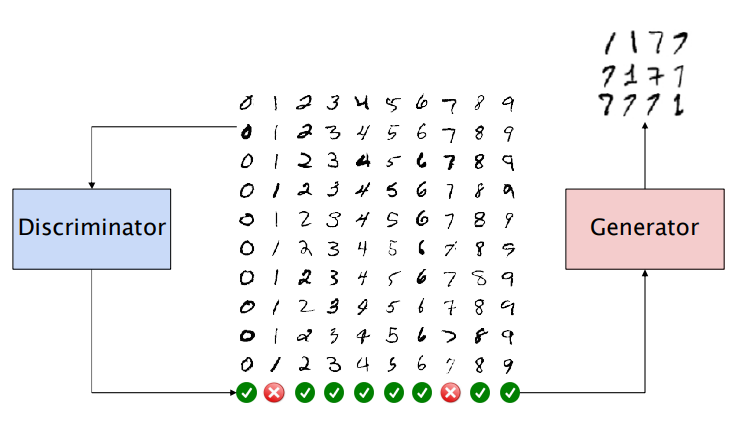
\includegraphics[scale=0.6]{img/mode.png}
    \caption{Mode collapse phenomenon}
\end{figure}

Just for mention them, three metrics to measure mode collapsing are: \textit{Inception Score}, \textit{Frechet Inception distance} and the more trivial but intuitive one is the \textit{Visual Inspection}.
Possible approaches to mitigate this issue are: 
\begin{itemize}
    \itemsep-0.3em
    \item Using a multiclass classification instead of a binary one (real/fake), it was empirically proven that it generates better samples there is not a formal proof; 
    \item Use \textit{different loss functions} for example MSE(L2), Energy-based losse, Wasserstein Loss...
\end{itemize}

\section{From GAN to DCGAN}
The original Goodfellow paper used fully connected model for the generator and the discriminator, however this is not a good solution for images in which the features to consider are more and more. An intuitive idea is that we can substitute fully connected models with CNN which performs very much better with respect to simple FCN which could lead too \textbf{many parameters}.  While for the discriminator a classical CNN is used, for the generator a decoder model which uses \textit{deconvolutions} and \textit{linear interpolation} is used. In the figure is showed a sketch for the generator architecture that from a noise vector in the latent space of 100 elements produces in output a generated  image $64\times64$.

\begin{figure}
    \centering
    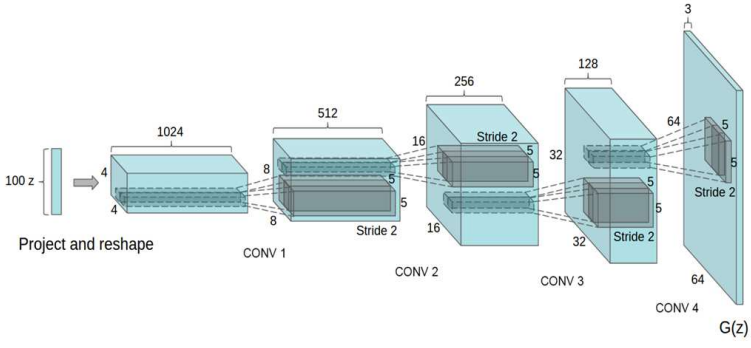
\includegraphics[scale=0.6]{img/DCGAN_generator.png}
    \caption{Example for DCGAN generator architecture}
\end{figure}

\section{Improving GAN}
Till now we have considered only unconditional generation, in which the generator starting from the noise vector $z$ does not have control over the generated data without any additional information.
However, there are cases in which one is interested into: (i) generate an example of a specific class within the ones present in the dataset, in this case we talk about \textbf{conditional generation}; (ii) given a generated example, have the possibility to modify some features looking for a way to manipulate/interpolate the latent space, in this case we are talking about \textbf{controllable generation}.

\subsection{Conditional GAN}
In this case both the architectures for \textit{Generator (G)} and \textit{Discriminator (D)} are slightly modified. The resulting model is called \textit{cGAN} (Conditional GAN). In particular, an extra information encoding either the class to generate (for G) or the class of which control the reality (for D), must be taken into account. Mostly, this information is passed to the GAN by using a \textit{one-hot encoding} like the one used in recurrent models. For example, if we have three classes and we want to generate/discriminate a sample for the first class the one-hot encoding is [1,0,0].

\subsubsection{Conditional Generator}
The generator takes as input the noise vector $z$ and the one-hot encoded label $y$ for the class to generate. 

\begin{figure}[h]
    \centering
    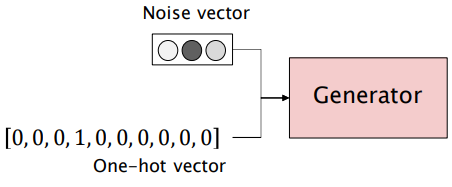
\includegraphics[scale=0.8]{img/condGen.png}
    \caption{Generator in cGAN}
\end{figure}

\subsubsection{Conditional Discriminator}
In the cGAN arcitecture the discriminator given the generated sample (or the real sample) outputs a probability for that image to be real or fake.

The overall architecture is shown in the following:

\begin{figure}
    \centering
    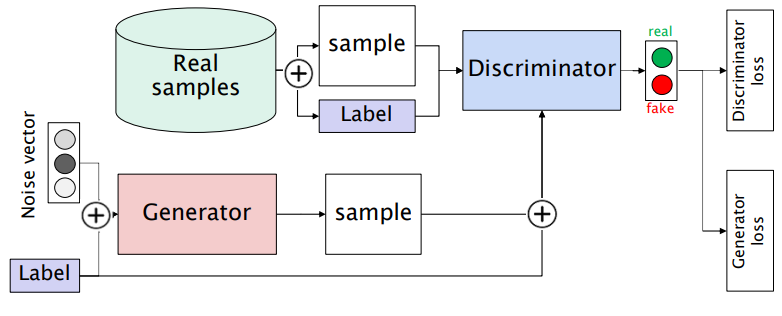
\includegraphics[scale=0.8]{img/cGAN.png}
    \caption{Complete cGAN architecture}
\end{figure}

\subsection{Controllable GAN}
We talk about \textbf{controllable generation} when we would like to change, in some way, given a generated image some features by acting on the latent space of the provided noise vector. Just for give an example, if the generator can generate faces, we want a way to change the age, the gender, the pose\dots \textbf{How to do this?} Now we are going to mention two methods for controllable generation whose common denominator is the effort in finding a way to associate dimensions of the latent space with generated examples.

\begin{figure}
    \centering
    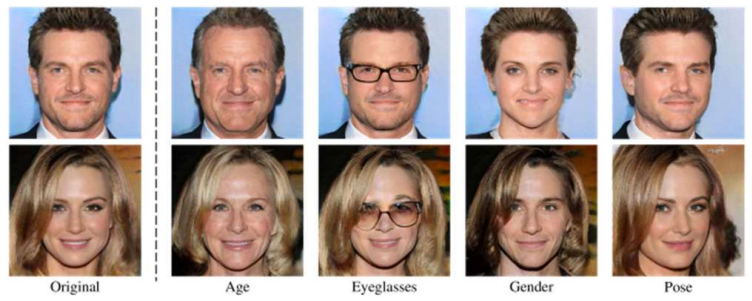
\includegraphics[scale=0.7]{img/contGAN.png}
    \caption{Example of controlled generated examples}
\end{figure}

\subsubsection{Interpolation in the $z$-space}
Here we consider for simplicity a 2D latent space. You start from two different noise vector (taken from a certain latent distribution eg. Gaussian, Normal...) and fed them into the generator we obtain two images $G(z_1)$ and $G(z_2)$ where $z_1$ and $z_2$ are the input noise vectors. In the bidimensional latent space this individuate a point. If we interpolate such points in the simplest way, by joining them with a segment we can obtain intermediate images between $G(z_1)$ and $G(z_2)$, by observing them we can obtain an intermediate generated image. Mathematically speaking the intermediate point is obtained as
\begin{equation*}
    z_{interp}=\alpha z_1 + (1-\alpha) z_2 \quad \alpha \in [0,1]
\end{equation*}
where $\alpha$ is an hyperparameter to control the position between the two points.

\begin{figure}
    \centering
    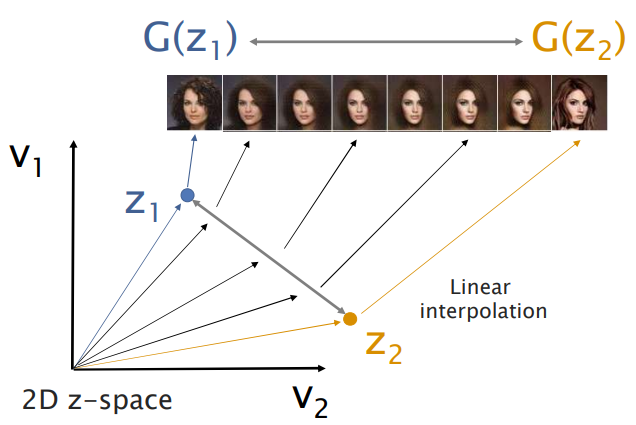
\includegraphics[scale=0.8]{img/interpz.png}
    \caption{Interpolation of the latent space}
\end{figure}

\subsubsection{Latent Direction for Feature control}
An even more interesting approach for control the generation is given the latent space (which is in general \textit{hyperdimensional}) look for \textbf{directions} along which you can move to change the particular feature it is associated to. For example, in the case I had a dog images generator, I would like to have the possibility to understand that moving across a certain directioni I can change the fur color for that generated dog. For example if you add a certain direction $v$ to the noise vector $z$ and the image $G(z)$ is added with a smile, this means that along such a direction you can \textit{control} the feature related to the smile. In formulae:
\begin{equation*}
    z_{mod}=z+\alpha v_{att}
\end{equation*}
where $v_{att}$ is the direction along which you control the attribute $att$ and $\alpha$ is to control the strength of that attribute.

\begin{figure}[h]
    \centering
    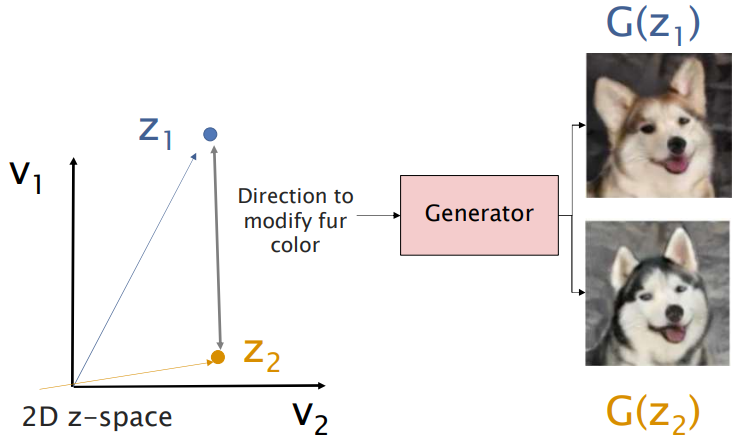
\includegraphics[scale=0.6]{img/directCont.png}
\end{figure}

The ideas we have just presented seem to be trivial, however there are some issues to manage.

\subsubsection{Output feature correlation}
The features of the output examples are sometimes strongly correlated so that if you act on a feature you also act on another correlated feature. Suppose you have an image $G(z)$ of a woman face, you want to add beard. It is very likely that modifying the direction of the beard will result in changing also the gender of the generated face, since usually (in the samples used for training the GAN) the woman have no beard. Then, it is quite difficult to \textbf{isoltate effects on the output}.

\subsubsection{Z-space entanglement}
It is likely that, given the input noise vector to a certain subset of elements are associated multiple features, since in general the number of features is much higher with respect to the dimension of the latent space. This problem is present even if all of the features of a certain image are all uncorrelated, here the cause of the problem stays in the latent space structure. This is the same to say that the $z$-space is \textbf{entangled}. How to solve this problem? One of the dummiest approaches the \textit{Supervised latent manipulation} in which more annotation to the images are added, but it is not convenient. Sometimes we struggle in obtaining the "basic" class labels! Here the solution is to increase the dimension of the latent space and add a \textit{regularizer} (supervised or unsupervised) to penalize the entanglement, obtaining a novel loss function made up as:
\begin{equation*}
    \mathcal{L}_{new}=\mathcal{L}_{adversarial} + \lambda \cdot \mathcal{L}_{regularizer}
\end{equation*}
a possible way is to maximize the \textbf{mutual information} (that is the statistical dependence between variables) so that could be a relation between the variables $z_i$ and the generated $G(z_i)$.\\

So far we have seen different ways to modify the "basic" GAN architecture in order to \textbf{condition the generated output} (by using additional information), to \textbf{control the generated output features} by structurally acting on the latent space. The remaining part of this chapter is devoted to present possible applications of GANs giving some examples of the most popular models for image-to-image translation, image super-resolution and tridimensional generation.




\section{Applications of GAN: Image-to-Image translation}
\textbf{Image-to-image translation} is one possible application for Generative Adversarial models, we have discussed so far, that deals with transferring the \textit{style} from one image to another keeping unchanged its \textit{content}. This is the underlying idea \textbf{image colorization} and \textbf{sketch to photo}. The methods for image-to-image (i2i) translation are split mainly in two groups:
\begin{enumerate}
    \itemsep-0.2em
    \item \textsf{Paired}: in this case each image in a domain has  the corresponding target image in the other domain; 
    \item \textsf{Unpaired}: such models two sets of unpaired data, the challenge is to find a way to transfer to a domain the main features of the other and viceversa.
\end{enumerate}

\begin{figure}[h]
    \centering
    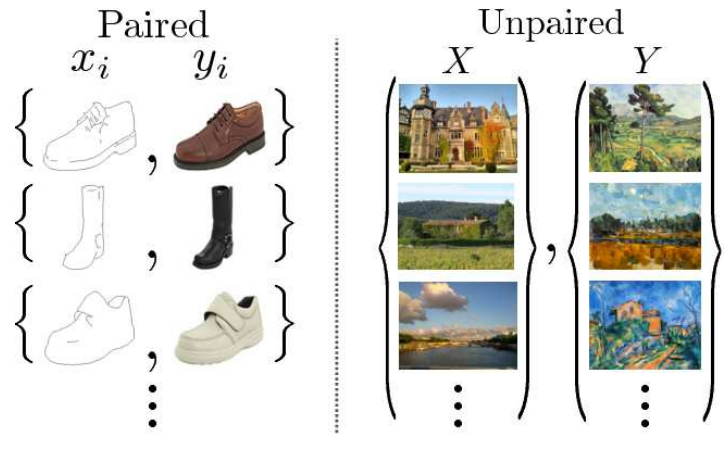
\includegraphics[scale=0.5]{img/pairedunpaired.png}
    \caption{Paired and Unpaired sets of images}
\end{figure}

\subsection{Pix2Pix architecture (Paired domains)}
This is a popular model for i2i, and is a type of conditional generation. In particular \textbf{Pix2Pix} involve two different domains: Sketches and Photos. The aim of the model is to translate the sketches into a photorealistic example. On the other hand, the discriminator takes as input the real input (sketch) concatened either with the generated output or the ground truth (the corresponding paired image). Note that here instead of the usual noise vector $z$ we have an image, however you can include also a noise vector in order to control the output features.

\begin{figure}
    \centering
    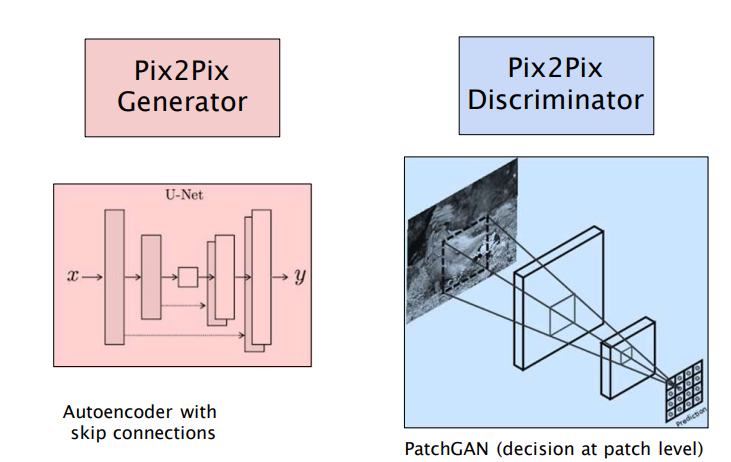
\includegraphics[scale=0.6]{img/pix2pix_arch.png}
    \caption{Pix2Pix architecture}
\end{figure}
What about the architecture of such a model? The \textbf{Generator} is a U-Net autoencoder, this first compress the image in a feature vector and then expands it to a generated image. On the other hand in order to improve the training of the GAN, a  \textbf{PatchGAN} is used for the discriminator, this instead of classifying the entire  image as real or fake, takes several patches of the input image and outputs a grid of probability for the patches to be associated with a real or a fake example.By doing this the learning process can be focused into iteratively improving particular regions of the images to be generated in order to win the minimax (on a certain extent) game. The Loss is composed by the \textit{adversarial loss} plus a regularization term

\begin{equation*}
    \mathcal{L}_{Pix2Pix} = 
    \mathcal{L}_{adversarial} + \lambda \mathcal{L}_{pixel}
\end{equation*}
where the term related to regularization is
\begin{equation*}
    \mathcal{L}_{pixel} = \sum_{i=1}^n \vert \text{generated}-\text{real} \vert
\end{equation*}

\subsection{Cycle GAN (Unpaired domains)}
\textbf{CycleGAN} is also a popular model for i2i \underline{unpaired} image translation, this architecture aims at finding a mapping between two sets of images (with different styles). For example, you want to turn a zebra into an horse and viceversa, tranpose an image of a season into another... Again, \textbf{How to do this?}

Suppose we have two different domains: Zebras and Horses. Since I start from completely separated domains, if from a source I apply the transformation $G$ we are obtaining a target (\textit{cycle}), if starting from the target I apply $F$, ideally the so generated image (ideally) must be the same with respect to the source (\textit{cycle consistency}).

\begin{figure}[h]
    \centering
    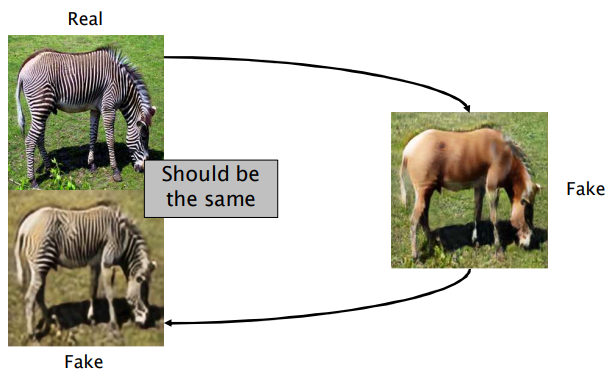
\includegraphics[scale=0.7]{img/cyclecons.png}
    \caption{Example of cycle consistency: starting from the zebras domain, we obtain an horse. The cycle consistency is satisfied if coming back I obtain the same zebra}.
\end{figure}

\noindent
Summarizing the cycle must guarantee the following, given the source $x$: 

\begin{equation*}
    x \to G(x) \to F(G(x)) \approx x 
\end{equation*}

In order to implement \textit{CycleGAN} we have to use two different GANs: one that transforms images from \textit{domain A} to \textit{domain B}, the other converting the images from \textit{domain B} to \textit{domain A}. The architecture of such GANs are identical to the one we have seen in the case of Pix2Pix. In CycleGAN we have that: (i) cicle consistency preserve the contents of a certain image; (ii) the discriminator loss guarantees the style transfer among different domains. How you can imagine, there will be a term in the loss function (common for the two GANs) which takes into account the cycle consistency, here such term is based on \textbf{pixel differences} in both loop directions. Here the adversarial loss is least-squares based (this help with vanishing gradient and mode collapse issues): 
\begin{equation*}
    \begin{cases}
        \mathbb{E}_x[(D(x)-1)^2]+\mathbb{E}_z[(D(G(z))-0)^2]&\textsf{Discriminator}\\
        \mathbb{E}_z[D(G(z)-1)^2]&\textsf{Generator}
    \end{cases}
\end{equation*}
\noindent
There is an (optional) extra loss term to help color preservation in the output, in order to guarantee this we can observe that a sample from domain A processed by the OPPOSITE (\textit{domain B}$\to$\textit{domain A}) must remain the same. This term is called \textbf{identity loss} and is the same as in pixel loss, the difference between the input and the real output. The resulting \textit{CycleGAN loss} is the following:
\begin{equation}
    \mathcal{L}_{cycleGAN}=\mathcal{L}_{adversarial}+\lambda_1{\mathcal{L}_{cycle_consistency}}+\lambda_2{\mathcal{L}_{identity}}
\end{equation}
All the terms must be duplicated to consider both GANs together, the training of such models occurs jointly: the two GANs are trained jointly. Another remark is to use CycleGANs when they can solve your problem (style transfer between images without changing the content). If you want translate a cat into a dog, do not use CycleGAN, since this involves \textit{geometric transformation}.

\section{Applications of GAN: Images Super-resolution}
Here the objective is to add some information to some image by creating new pixel contents. The most popular model for image Super-Resolution (SR) is \textbf{SRResNet}. They are DCGAN like architecture. During the training fase some high resolution (HR) images are downsampled to obtain a low-resolution (LR) one. Such an LR is fed to a \textit{generator} which creates a super-resolution (SR) of LR. In this case the \textit{discriminator} evaluates if we were able to add the lost information in domwnsampling the HR image.

\begin{figure}[h]
    \centering
    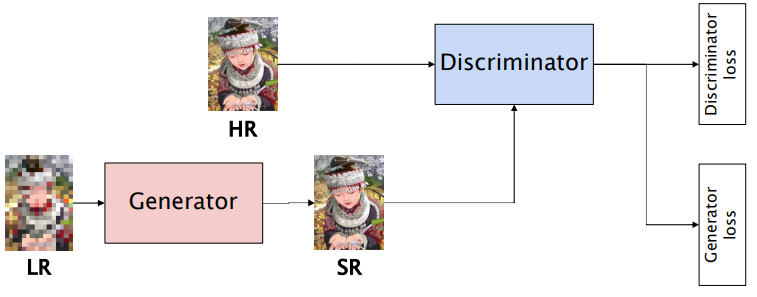
\includegraphics[scale=0.8]{img/SRResNet.png}
    \caption{Image Super-Resolution architecture}
\end{figure}

The \textit{discriminator loss} is a standard BCE (Binary Cross Entropy) loss, while the \textit{generator loss} is the sum of the standard adversarial log-loss and a \textsf{content loss} which aims at minimizing the perceptual loss \textbf{between HR and SR}, is used VGG-19 as feature extractor, an Mean Squared Error loss is used between the features of the last layer of extracted from VGG and the first features of the generator before being upsampled to the super-resolution image. See the conference paper \textit{\citetitle{ledig2017photo}} by \citeauthor{ledig2017photo}, \cite{ledig2017photo} fur further details.

\section{Applications of GAN: 3D GAN}
What if instead of 2D images we want to generate 3D objects? The approach remains the same: a generator creates 3D shapes a discriminator tells real from fake 3D models. How it is shown in \Citeauthor{wu2016learning}, \cite{wu2016learning}, the generated object lies in a \textit{voxel\footnote{
    The voxel is the counterpart of the pixel for 3D objects.
} space}. How you can imagine there is high unbalance between the generator and the discriminator: is much simpler to understand whether an object is real or fake; on the other hand the generator must create from a noise vector a tridimensional shape! For these reasons, there are some training tricks, you can adopt when training a model like this:
\begin{enumerate}
    \itemsep-0.3em
    \item Learning rate for D is much smaller than the one in G; 
    \item Batch size is very large;
    \item Discriminator weights are updated only if the accuracy in the last batch is less than 80\%.
\end{enumerate}
There are some techiniques which uses a VAE (Variational  Autoencoders) in conjuction with 3D-GAN since this ensure that similar latent vector originates similar 3D outputs, making the generation process \textit{more interpretable} and \textit{predictable}.